\documentclass[UTF8, a4paper]{ctexart}
\usepackage[margin=1in]{geometry} % 页边距调整
\usepackage{ctex}
\usepackage{array, amsmath, amssymb}

\usepackage{booktabs, tabularx, multirow, multicol} % 表格拓展支持
\usepackage{graphicx, subfigure, float} % 图片排版支持

\usepackage{algorithm, algpseudocode} % 伪代码支持
\renewcommand{\algorithmicrequire}{\textbf{Input:}}  
\renewcommand{\algorithmicensure}{\textbf{Output:}} 

\usepackage{tikz, mathpazo} % 基本绘图支持
\usepackage{flowchart} % 流程图支持
\usepackage{pgf-umlcd} % UML类图支持
\usetikzlibrary{arrows, shapes, chains, shapes.geometric}

\usepackage{listings} % 代码块支持
\usepackage{xcolor}
\lstset{
	language		= c++,
	backgroundcolor	= \color{white},
	basicstyle		= \footnotesize\ttfamily,
	keywordstyle	= \color{blue},
	stringstyle		= \color{red!58!blue!82}\ttfamily,
	commentstyle	= \color{darkgray},
	rulesepcolor	= \color{red!20!green!20!blue!20},
	columns			= fullflexible,
	breaklines		= true,
	captionpos		= b,
	tabsize			= 4,
	frame			= single,
	escapeinside	= {\%*}{*)}
}
%%示例
% \begin{lstlisting}[caption={}]
% #include <iostream>
% int main(int argc, char *argv[]) {
% 	std::cout << "Hello World!" << std::endl;
% 	return 0;
% }
% \end{lstlisting}

\usepackage{datetime} %日期
\renewcommand{\today}{\number\year{年}\number\month{月}\number\day{日}}

\begin{document}

\begin{center}
	\zihao{3}《数据结构》实验报告
\end{center}
\zihao{5}

\newcolumntype{Y}{>{\raggedleft\arraybackslash}X}
\noindent\begin{tabularx}{\textwidth}{XcY}
	  {班 级:}\;\underline{DL062123}
	& {姓 名:}\;\underline{项乔栋}
	& {学 号:}\;\underline{2021302468} \\
	  {邮 箱:}\;\underline{13282135976@sina.cn}
	& {日 期:}\;\underline{\today}
	& {编 号:}\;\underline{DS08}
\end{tabularx}
~\\

\noindent\textbf{$\circledcirc$
实验题目:\quad{单源最短路径长度}} \par
\noindent\textbf{$\circledcirc$
实验目的:\quad{解决图论问题}} \par
\noindent\textbf{$\circledcirc$
实验内容:\quad{自选算法实现单源最短路径长度的求解}} \par

\subsection*{一、需求分析}
\noindent\fbox{
\begin{tabularx}{\textwidth}{lY}
\bf{Description}
& \parbox[t]{\linewidth}{
	给一个赋权图(无向图),求0号结点到其余结点的最短路径的长度。
} \\

\bf{Input}
& \parbox[t]{\linewidth}{
	先输入一个小于等于100的正整数n,然后输入赋权图的邻接矩阵(10000表示无穷大,并且任意一条简单路径的长度都小于10000)。
} \\

\bf{Output}
& \parbox[t]{\linewidth}{
	按结点编号顺序输出0号结点所有结点的最短路径的长度。
} \\

\bf{Sample Input}
& \fbox{\parbox[t]{\linewidth}{\bf{
	\mbox{6} \\
    \mbox{0     1     4 10000 10000 10000} \\
    \mbox{1     0     2     7     5 10000} \\
    \mbox{4     2     0 10000     1 10000} \\
	\mbox{10000     7 10000     0     3     2} \\
	\mbox{10000     5     1     3     0     6} \\
	\mbox{10000 10000 10000     2     6     0}
}}} \\

\bf{Sample Output}
& \fbox{\parbox[t]{\linewidth}{\bf{
	\mbox{0} \\
	\mbox{1} \\
	\mbox{3} \\
	\mbox{7} \\
	\mbox{4} \\
	\mbox{9}
}}}
\end{tabularx}}

\subsection*{二、概要设计}
% 摘要
\par
1.\;基本操作: \par
	CreateFromIO() $\rightarrow$ Graph \par
	\qquad\textbf{操作结果:}\;从IO流创建无向图 \par
	BFS(G:Graph) $\rightarrow$ Array<Integer> \par
	\qquad\textbf{操作结果:}\;BFS求解单源最短路径长度 \par
2.\;程序模块: \par
1) 主程序 \par
2) IO支持 \par
3) BFS SSSP问题求解 \par
\begin{figure}[H]
	\begin{minipage}[t]{\linewidth}
		\centering
		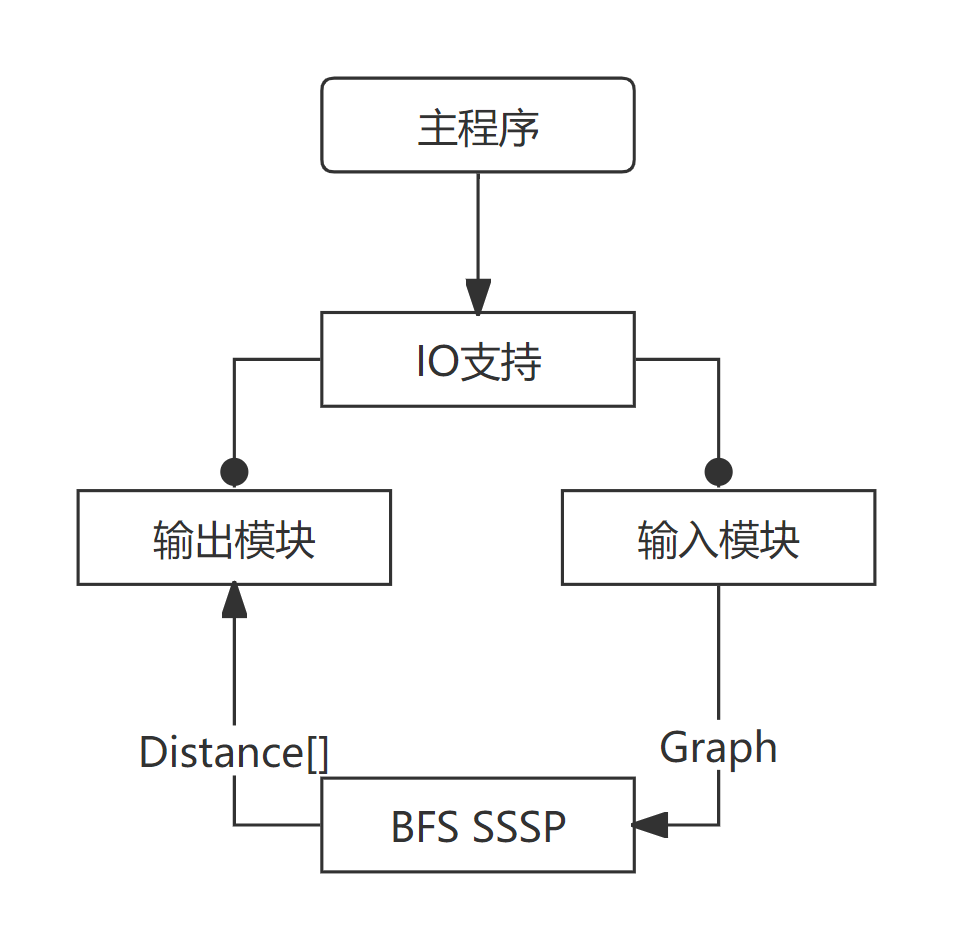
\includegraphics[width=80mm,height=85mm]{./assets/DS08-1}
	\end{minipage}
\end{figure}

\subsection*{三、详细设计}
\begin{algorithm}[H]
\begin{algorithmic}[1]
\caption{SSSP Solution Based on BFS}
\Require UG: $\mathbf{G}$
\Ensure Array<Integer>: $\mathbf{distance}$
\State let Q $\gets$ PriorityQueue<from,to,weight>
\While {not all vertices are visited}
	\State extract minimum edge from Q as e
	\State visit(e.to)
	\State let $\mathbf{distance}[e.to]$ $\gets$ e.weight
	\For {all unvisted connected vertex of e.to}
		\State Q.push({from: e.to, to: vertex, weight: e.weight + G[e.to][vertex]})
	\EndFor
\EndWhile
\State return $\mathbf{distance}$
\end{algorithmic}
\end{algorithm}

\subsection*{四、使用说明、测试分析与结果}
\subsubsection*{1、使用说明}
1) 本程序可以通过任意支持C++11及以上标准的编译器生成目标文件并在当前平台运行。 \par
2) 进入程序后务必依照需求的输入样式输入数据,手动输入与流式输入都是被允许的。 \par
\subsubsection*{2、测试结果与分析}
2.1\;\textbf{实际环境} \par
对于所有输入,皆为正赋权无向图,且满足输入要求中提及的条件。 \par
2.2\;\textbf{边界情况} \par
无 \par
2.3\;\textbf{测试结果} \par
目标代码通过全部测试,无需纠正 \par
\subsubsection*{3、调试过程问题分析与解决办法}
编码与测试环节皆未产生必须被处理的问题,跳过调试环节 \par
\subsubsection*{4、设计与实现的回顾讨论与分析}
给定题目并未要求必须使用何种算法进行求解,且只需计算最短路径长度,无需额外存储最短路径,故以BFS形式利用STL的优先队列进行Dijkstra算法的编写,算法流程较为清晰,避免了不必要的错误与调试的必要。 \par
\subsubsection*{5、运行界面}
\begin{figure}[H]
	\begin{minipage}[t]{\linewidth}
		\centering
		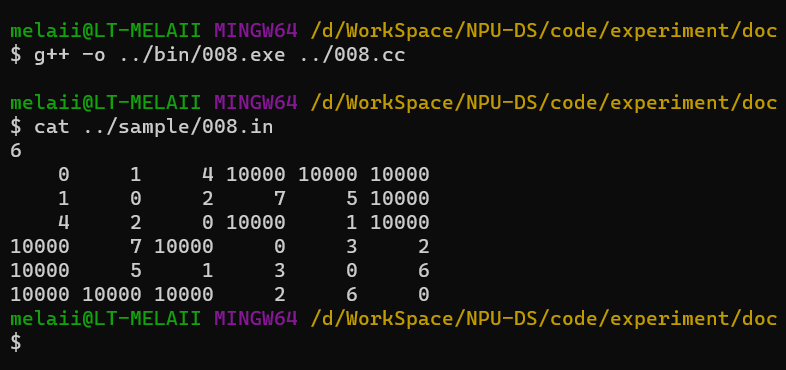
\includegraphics[width=125mm,height=60mm]{./assets/DS08-2}
		\caption{前置环境}
	\end{minipage}
\end{figure}
\begin{figure}[H]
	\begin{minipage}[t]{\linewidth}
		\centering
		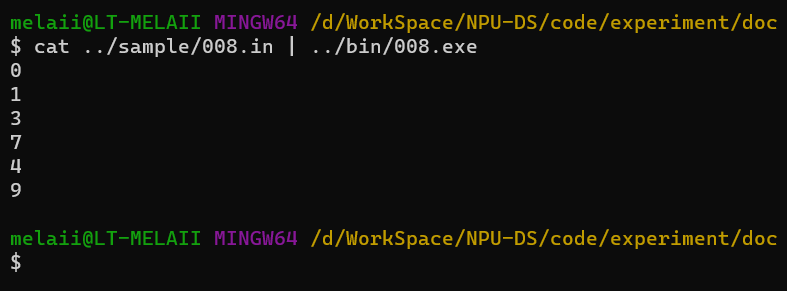
\includegraphics[width=125mm,height=48mm]{./assets/DS08-3}
		\caption{结果输出}
	\end{minipage}
\end{figure}

\subsection*{五、实验总结}
单源最短路径作为一个传统的图论问题,其对应的算法也是极为经典。且该实验并未给多余的要求,故明面上并无太多值得讨论的地方,整体来说算是对Dijkstra算法具体实现代码的一次练手。

~\\
\zihao{-4}
\textbf{教师评语:}
~\\
\textbf{实验成绩:}

\begin{flushright}
\mbox{指导教师签名:\qquad\qquad} \\
\mbox{批阅日期:\qquad\qquad}
\end{flushright}

\end{document}